% Created 2023-09-08 Fri 17:12
% Intended LaTeX compiler: pdflatex
\documentclass[11pt]{article}
\usepackage[utf8]{inputenc}
\usepackage[T1]{fontenc}
\usepackage{graphicx}
\usepackage{longtable}
\usepackage{wrapfig}
\usepackage{rotating}
\usepackage[normalem]{ulem}
\usepackage{amsmath}
\usepackage{amssymb}
\usepackage{capt-of}
\usepackage{hyperref}
\usepackage{minted}
\usepackage[a4paper]{geometry}
\usepackage{mathtools}
\author{Alexander Huss}
\date{\today}
\title{NLO calculations: Subtraction and Slicing}
\hypersetup{
 pdfauthor={Alexander Huss},
 pdftitle={NLO calculations: Subtraction and Slicing},
 pdfkeywords={},
 pdfsubject={},
 pdfcreator={Emacs 29.1 (Org mode 9.7)}, 
 pdflang={English}}
\begin{document}

\maketitle
\tableofcontents



\section{Introduction}
\label{sec:org97aa8b4}
Let us study a simple toy example for an NLO calculation and investigate what challenges arise in the context of fully differential predictions.
We will further have a look at two strategies to implement the IRC calcellation differentially: local subtractions and slicing.
These will be contrasted in their respective properties and performance.

\section{Inclusive calculation}
\label{sec:org2bc3730}
Let us first set the stage by considering our toy example in an \emph{inclusive} setup, i.e. where we have no restrictions on the phase space whatsoever (think: total cross section).
We use dimensional regularization (\(D=4-2\epsilon\)) to regulate all divergences and will drop all terms \(\mathcal{O}(\epsilon)\) in the expressions that follow.
We further assume that the Born kinematics is fully constraint such that they do not involve any integration.
The only term with a ``phase-space'' integration is therefore the real contribution, for which we assume a very simple integration domain \(x\in[0,\,1]\) (the limit of no emission given by \(x\to0\)).

With these considerations in place, let's fix the expressions for the virtual (``V'') and real-emission (``R'') contributions
\begin{align}
\label{eq:inc}
  \sigma^\mathrm{V}_\mathrm{inc.}
  &=
  \frac{1}{\epsilon} + a
  \,, &
  \sigma^\mathrm{R}_\mathrm{inc.}
  &=
  \int_0^1\mathrm{d}x\,\frac{1+bx}{x^{1+\epsilon}}
  =
  -\frac{1}{\epsilon} + b
  \,,
\end{align}
where we have explicilty performed the real-emission integral and dropped terms of \(\mathcal{O}(\epsilon)\).
We can appreciate how the singularities (poles in \(\epsilon\)) cancel between the virtual and real corrections (by construction) and the NLO corrections for the inclusive case simply read
\begin{align}
  \sigma^\mathrm{\delta NLO}_\mathrm{inc.}
  &=
  \sigma^\mathrm{V}_\mathrm{inc.} +
  \sigma^\mathrm{R}_\mathrm{inc.}
  =
  a+b
\end{align}

\section{Differential predictions}
\label{sec:org26b44f5}
In a differential setup we want to admit arbitraty (IRC safe) measurement functions to act on the phase space.
Since in this simple toy example the Born phase space is fully constrained, this means we have to allow for an arbitrary function to appear in the integrand of the real corrections and the virtual piece only gets multiplied by that function in the Born limit, i.e. \(x\equiv0\).
In summary, the pieces we need to evaluate are, c.f. Eq. \eqref{eq:inc},
\begin{align}
\label{eq:diff}
  \sigma^\mathrm{V}_\mathrm{diff.}
  &=
  \biggl( \frac{1}{\epsilon} + a \biggr) \;\mathcal{J}(0)
  \,, &
  \sigma^\mathrm{R}_\mathrm{diff.}
  &=
  \int_0^1\mathrm{d}x\,\frac{1+bx}{x^{1+\epsilon}}
  \;\mathcal{J}(x)
  \,.
\end{align}
The main point here is that \(\mathcal{J}(x)\) can in general be very complicated (think: isolation algorithms, jet clusterings, energy-energy correlators, \ldots{}) such that tackling this integral analytically is inpractical.
Moreover, you do not want to re-compute a difficult integral each time the measurement function changes.

From these considerations it becomes apparent that we'll want a flexible \emph{numerical} way of evaluating this integral.
The main challenge we then face is that the real-emission integral is actually divergent, which is why we had to introduce a regulator (note that in general, we'll be facing \(D=4-2\epsilon\) dimensional integrals, which are non-integer and thus not suitable for a Monte Carlo approach).
To expose the singularity, we need to perform some (partial) integration of the real-emission phase space, but at the same time we want to remain fully differential in the kinematics, i.e. want to keep the integration in tact.
These seemingly contradicting requirements are what is sloved using so-called \emph{subtraction methods}, which rearrange the divergences so we end up with only well-defined (finite) integrals that we can do numerically.

\subsection{Local Subtraction}
\label{sec:org30ac1cf}
The local subtraction follows a very common strategy in solving physics problems: find a suitable prarametrisation of a zero.
We essentially subtract something differentially and add the same quantity back in integrated form.
For this to work, we need a very good understanding of how the singularities arise in our calculations.
In real applications one exploits \emph{factorization} in the IRC limits to devise universal methods to deal with the singularities.

Here, the situation is very simple: the singularity comes from the \(x\to0\) limit of the real-emission integral.
So we can find a very simple prescription to isolate the singularity by rewriting the real-emission corresions as foloows
\begin{align}
  \sigma^\mathrm{R}_\mathrm{diff.}
  &=
  \int_0^1\mathrm{d}x\,\frac{1+bx}{x^{1+\epsilon}}
  \;\mathcal{J}(x)
  \nonumber\\&=
  \int_0^1\mathrm{d}x\,\frac{1+bx}{x^{1+\epsilon}}
  \;\Big[\mathcal{J}(x) - \mathcal{J}(0)\Bigr]
  + \mathcal{J}(0)
  \int_0^1\mathrm{d}x\,\frac{1+bx}{x^{1+\epsilon}}
  \nonumber\\&=
  \int_0^1\mathrm{d}x\,\frac{1+bx}{x}
  \;\Big[\mathcal{J}(x) - \mathcal{J}(0)\bigr]
  +\biggl( -\frac{1}{\epsilon} + b \biggr) \;\mathcal{J}(0)
  \,.
\end{align}
In the last step we set \(\epsilon=0\) in the first term, since it's now finite with the counterterm; the singularity is fully isolated in the second term that we could perform analytically independent of the measurement function.

Combining this with the virtual corrections, we can appreciate how a local subtraction manages to arrange the calculation into finite pieces that are amenable to numerical evaluation:
\begin{align}
\label{eq:subtr}
  \sigma^\mathrm{\delta NLO}_\mathrm{diff.}
  &=
  (a + b) \;\mathcal{J}(0)
  +\int_0^1\mathrm{d}x\,\frac{1+bx}{x}
  \;\Big[\mathcal{J}(x) - \mathcal{J}(0)\Bigr]
\end{align}

\subsubsection{Implementation}
\label{sec:orgbf4abc5}
The implementation of \eqref{eq:subtr} in a python function is straighforward.
We choose the VEGAS algorithm to integrate the real-emission ``phase space'' and give the number of calls (events) as an argument so wo can compare the performance later
\begin{minted}[frame=lines,fontsize=\scriptsize]{python}
def subtr_dNLO(ncall: int) -> tuple[float, float]:

    def integrand(x: list[float]) -> float:
        return (1. + b * x[0]) / x[0] * (J(x[0]) - J(0))

    integ = vegas.Integrator([[0, 1]])
    integ(integrand, nitn=10, neval=(ncall / 10))  # 10% into adaption
    result = integ(integrand, nitn=10, neval=ncall)

    return ((a + b) * J(0) + result.mean, result.sdev)
\end{minted}

\subsection{Non-Local Subtraction: Slicing}
\label{sec:org9bbd365}
In a non-local subtraction, or \emph{slicing} approach, one exploits the fact that the divergence can be isolated with some resolution variable on which we place a cut to regulate the divergence.
It is important to note that slicing methods are not ``exact'' but come with an error that must be controlled and estimated.

In this toy example, we already know that the singularity arises from the \(x\to0\) limit so we can regulate the real-emission integral by imposing \(x > \xi > 0\):
\begin{align}
  \sigma^\mathrm{R}_\mathrm{diff.}
  &=
  \int_0^1\mathrm{d}x\,\frac{1+bx}{x^{1+\epsilon}}
  \;\mathcal{J}(x)
  \nonumber\\&=
  \int_0^\xi\mathrm{d}x\,\frac{1+bx}{x^{1+\epsilon}}
  \;\mathcal{J}(x) +
  \int_\xi^1\mathrm{d}x\,\frac{1+bx}{x^{1+\epsilon}}
  \;\mathcal{J}(x)
  \nonumber\\&=
  \int_0^\xi\mathrm{d}x\,\frac{1+bx}{x^{1+\epsilon}}
  \;\Big[\mathcal{J}(0) + \mathcal{O}(\xi^n)\Bigr]
  +\int_\xi^1\mathrm{d}x\,\frac{1+bx}{x}
  \;\mathcal{J}(x)
  \nonumber\\&=
  \biggl( -\frac{1}{\epsilon} + \ln(\xi) \biggr) \;\mathcal{J}(0)
  +\int_\xi^1\mathrm{d}x\,\frac{1+bx}{x}
  \;\mathcal{J}(x)
  + \mathcal{O}(\xi^n)
  \,.
\end{align}
The crucial step is in the third line, where we expanded \(\mathcal{J}(x) \simeq \mathcal{J}(0) + \mathcal{O}(\xi^n)\), again allowing to pull out the measurement function out of the integral that diverges.
It also becomes clear that there's explicitly an \emph{error} that we make by expanding the measurement function this way and that we'll want to take \(\xi\) as small as possible.
However, we also see that the regulator induces a \(\ln(\xi)\) term that blows up as we take \(\xi\to0\) and we will see how that impacts the performance of the method later.
The power of the error term will depend on the parameter/observable we choose (\(x\)) and the measurement function \(\mathcal{J}\).

Combining the terms with the virtual corrections, we get the slicing result with the \(\xi\) \emph{cutoff} parameter
dependence and an associated error
\begin{align}
\label{eq:slice}
  \sigma^\mathrm{\delta NLO}_\mathrm{diff.}
  &=
  \bigl(a + \ln(\xi)\bigr) \;\mathcal{J}(0)
  +\int_\xi^1\mathrm{d}x\,\frac{1+bx}{x}
  \;\mathcal{J}(x)
  + \mathcal{O}(\xi^n)
\end{align}

\subsubsection{Implementation}
\label{sec:orgc10afca}
The implementation of \eqref{eq:slice} in a python function is analogous to the subtraction case above.
This time, we also have the cutoff parameter \(\xi\) as an argument as we'll want to vary it and see how the errors change.
\begin{minted}[frame=lines,fontsize=\scriptsize]{python}
def slice_dNLO(xi: float, ncall: int) -> tuple[float, float]:

    if (xi <= 0.) or (xi > 1.):
        raise ValueError("cutoff not in valid range [0,1]: {}".format(xi))

    def integrand(x: list[float]) -> float:
        return (1. + b * x[0]) / x[0] * J(x[0])

    integ = vegas.Integrator([[xi, 1]])
    integ(integrand, nitn=10, neval=(ncall / 10))  # 10% into adaption
    result = integ(integrand, nitn=10, neval=ncall)

    return ((a + math.log(xi)) * J(0) + result.mean, result.sdev)
\end{minted}



\section{Playground}
\label{sec:org4668aea}
Let us export the two approaches we introduced above and compare their performance.
For simplicity we'll set the constants in the virtual and real corrections to one
\begin{minted}[frame=lines,fontsize=\scriptsize]{python}
# the constants in the virtual and real corrections defined globally
a: float = 1.
b: float = 1.
\end{minted}
For the measurement function, we implement a few to test the dependence of the methods on it properties.
\begin{minted}[frame=lines,fontsize=\scriptsize]{python}
# the measurement function (global flag as switch)
iJ: int = 1
def J(x: float) -> float:
    if iJ == 0:
        # total cross section (= a + b)
        return 1.
    elif iJ == 1:
        # linear dependence => linear error term
        return 1. - x
    elif iJ == 2:
        # quadratic dependence & error
        return 1. - x**2
    elif iJ == 3:
        # a more complex one (quadratic)
        return math.cosh(x)
    else:
        raise RuntimeError(
            "unknown measurement function switch: {}".format(iJ))
\end{minted}

\begin{quote}
\begin{itemize}
\item Feel free to implement your own one here and try it out.
\end{itemize}
\end{quote}


\subsection{Export source code}
\label{sec:org528d21c}
We can export the python source code to a file \texttt{main.py}:
\begin{minted}[frame=lines,fontsize=\scriptsize]{python}
import math
import vegas
import numpy as np
import sys

# the constants in the virtual and real corrections defined globally
a: float = 1.
b: float = 1.

# the measurement function (global flag as switch)
iJ: int = 1
def J(x: float) -> float:
    if iJ == 0:
        # total cross section (= a + b)
        return 1.
    elif iJ == 1:
        # linear dependence => linear error term
        return 1. - x
    elif iJ == 2:
        # quadratic dependence & error
        return 1. - x**2
    elif iJ == 3:
        # a more complex one (quadratic)
        return math.cosh(x)
    else:
        raise RuntimeError(
            "unknown measurement function switch: {}".format(iJ))

def subtr_dNLO(ncall: int) -> tuple[float, float]:

    def integrand(x: list[float]) -> float:
        return (1. + b * x[0]) / x[0] * (J(x[0]) - J(0))

    integ = vegas.Integrator([[0, 1]])
    integ(integrand, nitn=10, neval=(ncall / 10))  # 10% into adaption
    result = integ(integrand, nitn=10, neval=ncall)

    return ((a + b) * J(0) + result.mean, result.sdev)

def slice_dNLO(xi: float, ncall: int) -> tuple[float, float]:

    if (xi <= 0.) or (xi > 1.):
        raise ValueError("cutoff not in valid range [0,1]: {}".format(xi))

    def integrand(x: list[float]) -> float:
        return (1. + b * x[0]) / x[0] * J(x[0])

    integ = vegas.Integrator([[xi, 1]])
    integ(integrand, nitn=10, neval=(ncall / 10))  # 10% into adaption
    result = integ(integrand, nitn=10, neval=ncall)

    return ((a + math.log(xi)) * J(0) + result.mean, result.sdev)

if __name__ == "__main__":
    if len(sys.argv) < 3:
        raise RuntimeError("I expect at least two arguments:  [subtr|slice]  ncall")
    ncall = int(sys.argv[2])
    if sys.argv[1].lower() == "subtr":
        res_subtr = subtr_dNLO(ncall=ncall)
        print("{:e} {:e}".format(*res_subtr))
    elif sys.argv[1].lower() == "slice":
        if len(sys.argv) == 6:
            ilow = int(sys.argv[3])
            iupp = int(sys.argv[4])
            nsteps = int(sys.argv[5])
        else:
            ilow = -3
            iupp = -3
            nsteps = 1
        res_subtr = subtr_dNLO(ncall=ncall)
        for xi in np.logspace(ilow, iupp, nsteps):
            res_slice = slice_dNLO(xi=xi, ncall=ncall)
            Del_val = res_slice[0] - res_subtr[0]
            Del_err = math.sqrt(res_slice[1]**2 + res_subtr[1]**2)
            print("{:e}  {:e} {:e}  {:+e} {:e}".format(
                xi, *res_slice, Del_val, Del_err))
    else:
        raise RuntimeError("unrecognised mode: {}".format(sys.argv[1]))
\end{minted}
by using the \texttt{tangle} command
\begin{minted}[frame=lines,fontsize=\scriptsize]{elisp}
(org-babel-tangle)
\end{minted}

Let's use the implementation to generate some ``events''
\begin{minted}[frame=lines,fontsize=\scriptsize]{shell}
python main.py subtr 1000            > data_subtr.dat
python main.py subtr 10000           > data_subtr_10.dat
python main.py subtr 100000          > data_subtr_100.dat
python main.py slice 1000   -4 -1 50 > data_slice.dat
python main.py slice 10000  -4 -1 50 > data_slice_10.dat
python main.py slice 100000 -4 -1 50 > data_slice_100.dat
\end{minted}
Time to plot the results; let up start with the \(N_\mathrm{call}=1000\) case:
\begin{center}
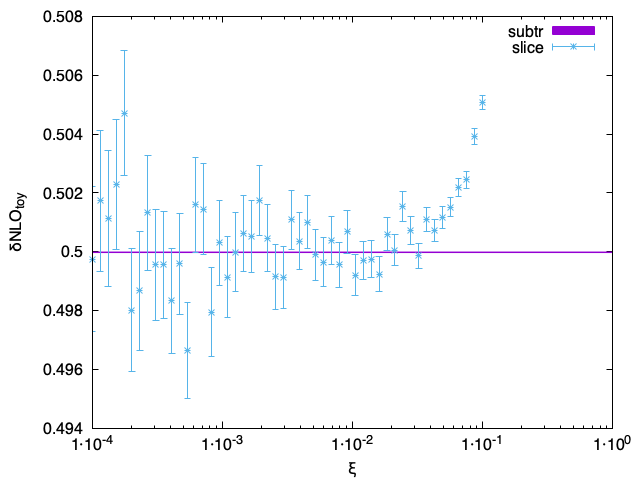
\includegraphics[width=.9\linewidth]{data.png}
\end{center}
We see that the local subtraction yields much smaller uncertainties than the slicing method for the same number of events.
We further see the error, which in this default setup is \emph{linear} \(\mathcal{O}(\xi)\), increases as we choose larger values of the cutoff.
Smaller \(\xi\) makes the results less stable; the reason is the large log \(\ln(\xi)\) in Eq. \eqref{eq:slice}, which must compensate against the cut-off regulated real-emission part.

From the plot, and the numerical accuracy we have achieved, the result starts to stabilize at around \(\xi \simeq 10^{-2}\).
However, this is a statement that depends on the accuracy target we have on the final result.
To make that point clear, let's look at the data with higher statistics and see how things compare

\begin{center}
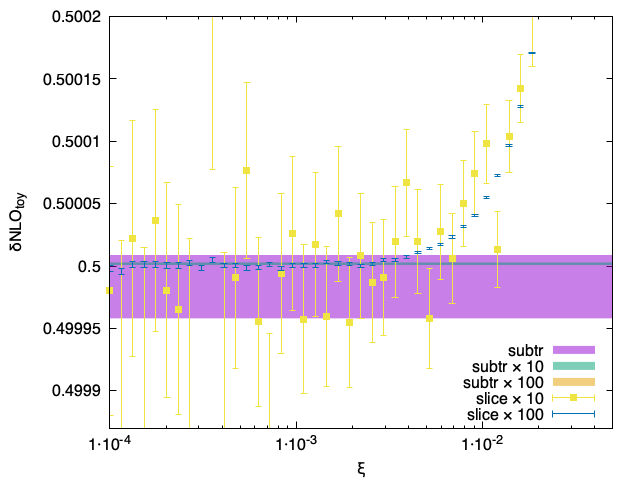
\includegraphics[width=.9\linewidth]{data_zoom.png}
\end{center}
For this specific example we see that we typically need \(\mathcal{O}(10)\) times more statistics in the slicing to achieve a similar numerical precision.
Note that in real-life application this can be much worse and also that there's an additional overhead of having to scan the \(\xi\) variation to find a ``plateau''.
With the numerical precision of ``slice \(\times\) 100'', we see that the \(\mathcal{O}(\xi)\) error only becomes subdominant below \(\xi \lesssim 10^{-3}\), that is to note that the smallness of the cutoff \(\xi\) is dictated by the target precision we aim for.

\begin{quote}
\begin{itemize}
\item Try to play around with different measurement functions; how does the picture change if the error is quadratic?
\end{itemize}
\end{quote}
\end{document}